\documentclass[12pt,twoside,openright,a5paper]{book}

\usepackage[a5paper]{geometry}

\usepackage{times}
\usepackage[Lenny]{fncychap}
%\usepackage[Conny]{fncychap}

\usepackage[spanish]{babel}
\usepackage[utf8]{inputenc}
\usepackage[T1]{fontenc}

\newcommand{\personaje}{Nombre del personaje}

\usepackage{mathptmx}
\usepackage{etoolbox}

\usepackage[titles]{tocloft}

\usepackage{fourier-orns}

\usepackage{graphicx}
\usepackage{float}

\usepackage{soulutf8} % para tachar palabras: \textst{tachame}

\usepackage{pdfpages}
\usepackage{afterpage}

\renewcommand{\cftchapleader}{\cftdotfill{\cftdotsep}}

\title{Xolopes}
\author{Juanjo Conti}
\date{}

\hyphenation{a-ttri-bu-tion}
\hyphenation{li-bre-rí-a}
\hyphenation{em-pe-za-ba}
\hyphenation{a-cos-tar-me}
\hyphenation{re-co-rrer}
\hyphenation{ma-yas}
\hyphenation{re-po-llo}
\hyphenation{per-dien-do}
\hyphenation{me-tros}
\hyphenation{di-si-mu-lar}

% Evitar viudas y huérfanas
\widowpenalty=10000
\clubpenalty=10000

\begin{document}

\pagestyle{plain}

\maketitle

\cleardoublepage

\thispagestyle{empty}
\noindent
Edición automágica. 2013.\\

\vspace{0.5cm}

\noindent
\emph{Xolopes} lleva la licencia 
Creative Commons Attribution - NonCommercial - ShareAlike 3.0 Unported License.
Esto significa que podés compartir esta obra y crear obras derivadas de la misma
mencionando al autor, pero no ha\-cer un uso comercial.

\vfill

\noindent
Más información sobre este libro:\\
http://www.juanjoconti.com.ar/xolopes\\

\noindent
Más libros del autor:\\
http://www.juanjoconti.com.ar/libros

\cleardoublepage

\noindent
\begin{flushright}
\emph{
\emph{Xolopes} \\está \\dedicado \\a \\mi \\papá \\y \\a \\mi \\mamá\\
que \\me \\enseñaron \\a \\leer \\y \\a \\amar.\\
\vspace{0.5cm}
Amo, por eso escribo.
}

\end{flushright}

\cleardoublepage

##CONTENT##

\vspace{0.5cm}
\hrulefill\hspace{0.2cm} \decofourright\decofourleft \hspace{0.2cm} \hrulefill

\cleardoublepage

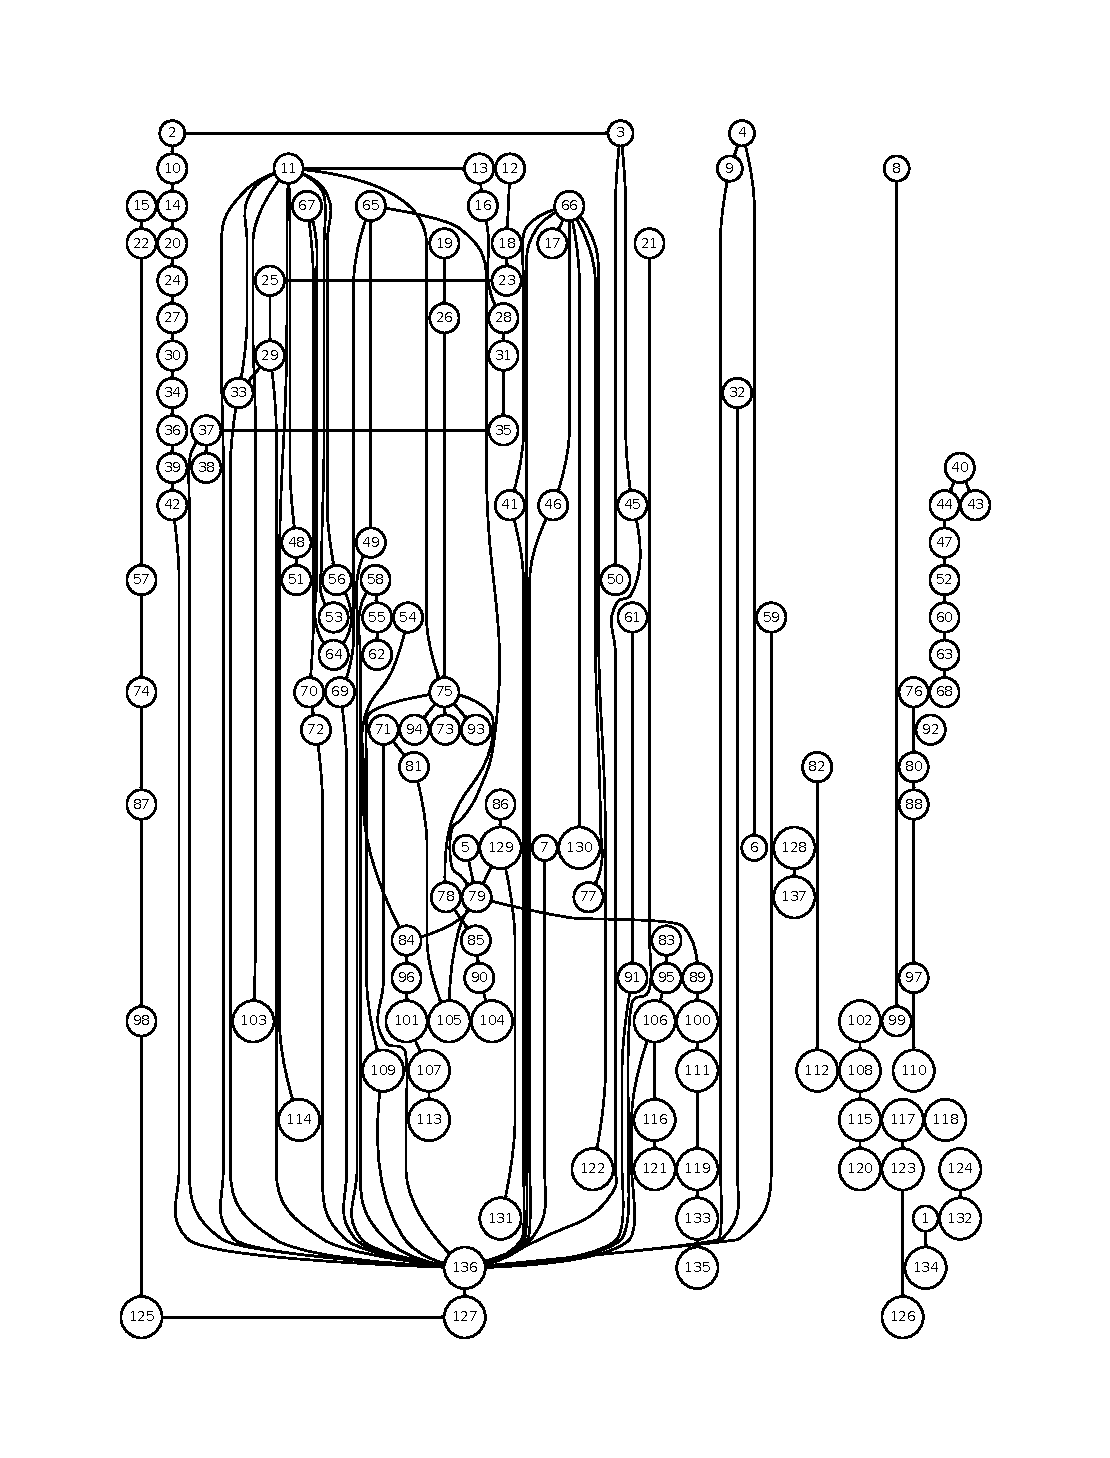
\includepdf{chunks.pdf}

\end{document}
